\section{Part 2.1: Original-Configuration SFT and Midtraining vs.\ Pretrained Model}

To address the first requirement of Part 2, we ran SFT and midtraining scripts starting from the same pretrained checkpoint and logged the runs in Weights \& Biases. 

\paragraph{Experimental setup.}
Both runs were initialized from the same pretrained checkpoint, \\
\texttt{nano-swiglu-fp8-full} at step 4357, ensuring that the comparison isolates the effect of the two training stages rather than differences in initialization. 
We selected the SwiGLU variant rather than the \texttt{nano-baseline-fp8-full} checkpoint because previous experiments in Assignment~3 showed that the SwiGLU architecture produces slightly stronger reasoning-oriented performance. 
Although the baseline model achieved marginally better language modeling efficiency (lower BPB), the SwiGLU variant obtained a higher CORE benchmark score (0.2086 vs.\ 0.2038), indicating modest improvements on reasoning and knowledge tasks despite slightly worse token-level prediction quality. 
This aligns with the broader literature where many modern LLMs (e.g., LLaMA, PaLM, Mistral) adopt SwiGLU activations to improve representational capacity for reasoning tasks. 
Because GSM8K primarily evaluates mathematical reasoning rather than raw language modeling quality, using the SwiGLU pretrained checkpoint provides a more appropriate starting point for downstream SFT and midtraining experiments.

The SFT and midtraining runs were executed using the original configuration files provided in the nanochat framework to ensure a controlled comparison with the pretrained checkpoint. 
Key hyperparameters for both stages are summarized in Table~\ref{tab:p2_training_configs}. 
Using the original configurations avoids introducing additional hyperparameter changes that could confound the comparison between the pretrained model, SFT, and midtraining.

\paragraph{Version Explain}
Karpathy removed the separate midtraining pipeline from nanochat in late January, which explains why we could not find the original midtraining script in the current codebase. Following the instructor clarification, we used the newest nanochat version and treated the updated chat SFT pipeline as the supported replacement. For comparability, we replaced the old midtraining stage with an additional 1000 training iterations under the current setup, which preserves the intent of giving the model more task-relevant post-pretraining exposure while staying aligned with the maintained upstream code rather than reviving an older deprecated version.

\begin{table}[H]
\centering
\caption{Original training configurations used for SFT and midtraining.}
\label{tab:p2_training_configs}
\begin{tabular}{p{2cm} p{3.2cm} p{2.2cm} p{6.2cm}}
\hline
\textbf{Stage} & \textbf{Parameter} & \textbf{Value} & \textbf{Justification} \\
\hline
SFT & device\_batch\_size & 8 & Chosen to fit GPU memory constraints during instruction-style supervised fine-tuning. \\

SFT & total\_batch\_size & 16,384 & Provides stable gradient estimates while maintaining reasonable training throughput. \\

SFT & attention\_impl & fa3 & Uses FlashAttention3 to improve attention efficiency and training speed. \\

SFT & render\_max\_tokens & 513 & Limits maximum generated response length during supervised instruction training. \\

\hline
Midtraining & depth & 20 & Matches the architecture of the pretrained nanochat model. \\

Midtraining & max\_seq\_len & 512 & Original context length used during nanochat pretraining. \\

Midtraining & device\_batch\_size & 32 & Larger batch per device improves hardware utilization during pretraining-style training. \\

Midtraining & total\_batch\_size & 1,048,576 & Large effective batch stabilizes optimization for large-scale token training. \\

Midtraining & MLP variant & SwiGLU & Maintains architectural consistency with the pretrained checkpoint. \\

Midtraining & precision & FP8 & Reduces memory usage and increases training throughput on modern GPUs. \\

\hline
\end{tabular}
\end{table}

\paragraph{Evaluation protocol.}
Although Part~2 of the assignment does not explicitly mandate a specific evaluation dataset, 
we evaluate all checkpoints on GSM8K to maintain consistency with the overall objective of 
the assignment, which is to improve mathematical reasoning performance on this benchmark. 
Using GSM8K at this stage provides an early diagnostic signal of whether SFT or midtraining 
changes the model’s ability to produce correct numerical answers before the RL phase. 
This allows us to establish a baseline comparison between the pretrained model, the SFT 
model, and the midtrained model under the same downstream evaluation that will later be 
optimized in Parts~3 and~4.

\paragraph{Evaluation criteria.}
We compare the models using four signals: training BPB, validation BPB, relaxed GSM8K numeric accuracy, and strict GSM8K exact-match accuracy(see \hyperref[sec:gsm8k_eval_def]{evaluation definition}). We also report parseable rate, since this helps explain whether a model is merely producing text or is actually emitting answers in a format that the evaluator can reliably score. This distinction is important here because downstream math performance depends not only on latent knowledge, but also on whether the model produces structured, numerically extractable completions.

\begin{table}[H]
\centering
\caption{Comparison of the pretrained checkpoint, original-configuration SFT, and original-configuration midtraining on GSM8K.}
\label{tab:p2_original_compare}
\begin{tabular}{l
                S[table-format=5.0]
                S[table-format=1.4]
                S[table-format=1.4]
                S[table-format=2.2]
                S[table-format=2.2]}
\toprule
\textbf{Model} & \textbf{Step} & \textbf{Train BPB} & \textbf{Val BPB} & \textbf{Strict Acc. (\%)} & \textbf{Relaxed Acc. (\%)} \\
\midrule
Pretrained & 4357  & 0.7824 & 0.7816 & 0.00 & 1.36 \\
SFT (original config) & 20444 & 1.5223 & 1.5242 & \bfseries 5.23 & \bfseries 6.37 \\
Midtraining (original config) & 5357 & \bfseries 0.7761 & \bfseries 0.7753 & 0.00 & 1.06 \\
\bottomrule
\end{tabular}
\end{table}


\begin{table}[H]
\centering
\caption{Output formatting quality on GSM8K measured by the parseable answer rate.}
\label{tab:p2_parseable}
\begin{tabular}{l S[table-format=2.2] l}
\toprule
\textbf{Model} & \textbf{Parseable Rate (\%)} & \textbf{Notes} \\
\midrule
Pretrained & 0.00 & Outputs are largely unstructured or non-extractable \\
SFT (original config) & \bfseries 73.16 & Strong improvement in answer extractability \\
Midtraining (original config) & 0.00 & No formatting improvement over pretrained \\
\bottomrule
\end{tabular}
\end{table}

\paragraph{Main result.}
The strongest result is that original-configuration SFT substantially improves GSM8K performance relative to the pretrained checkpoint. Relaxed numeric accuracy rises from 1.36\% to 6.37\%, an absolute gain of 4.99 percentage points and roughly a 4.7$\times$ relative improvement. More importantly, strict exact-match accuracy increases from 0.00\% to 5.23\%, and parseable rate rises from 0.00\% to 73.16\%. This indicates that SFT does more than slightly shift token probabilities: it changes the model's response format enough to make its mathematical outputs much more scorable and substantially more useful for downstream evaluation.

By contrast, original-configuration midtraining does \emph{not} improve downstream GSM8K performance. Although validation BPB improves slightly from 0.7816 to 0.7753, relaxed accuracy falls from 1.36\% to 1.06\%, strict accuracy remains at 0.00\%, and parseable rate also remains at 0.00\%. In other words, the midtraining run appears to improve the language-modeling objective without improving mathematical answer production.

\paragraph{Interpreting the BPB--accuracy trade-off.}
An important finding from this ablation is that lower BPB does not automatically imply better task performance. Midtraining achieves the best validation BPB of the three checkpoints, yet it does not translate into better GSM8K accuracy. SFT shows the opposite pattern: it significantly worsens BPB while dramatically improving GSM8K answerability and correctness. This divergence suggests that the two stages optimize for meaningfully different behaviors. The midtraining objective appears to improve next-token prediction under its training distribution, whereas SFT more directly teaches the model how to respond in a task-compatible format and how to produce concrete problem-solving traces that the GSM8K evaluator can parse.

This is exactly why both types of metrics should be reported. If we only looked at BPB, we would incorrectly conclude that midtraining is the best stage. If we only looked at final accuracy, we would miss the fact that SFT's gains come with a substantial language-modeling trade-off. Reporting both gives a more faithful picture of what each training stage actually changes.

\paragraph{Qualitative behavior.}
The qualitative samples reinforce the quantitative results. The pretrained checkpoint often produces repetitive or poorly grounded text and rarely emits a clean answer string. The midtrained model exhibits a similar failure mode: many completions remain repetitive, templated, or loosely related to the question, which is consistent with its zero parseable rate. In contrast, the SFT model frequently produces multi-step, calculator-style reasoning traces with explicit numeric manipulations, making its answers far easier to extract and score. However, many of these traces are still logically incorrect, which explains why SFT improves accuracy significantly but remains far from strong overall GSM8K performance.

\paragraph{ W\& B data.}
We include W\&B plots as evidence for optimization dynamics that are not visible from the final table alone. The SFT curves should be used to show that the run converged to a very different operating regime from the pretrained model, while the midtraining curves should show that its training objective improved smoothly even though downstream reasoning did not. These figures justify an important conclusion of this part: optimization success under the run's native loss is not sufficient evidence of improvement on GSM8K. The figures therefore support the interpretation of Table~\ref{tab:p2_original_compare} rather than merely repeating it.

\begin{figure}[H]
    \centering
    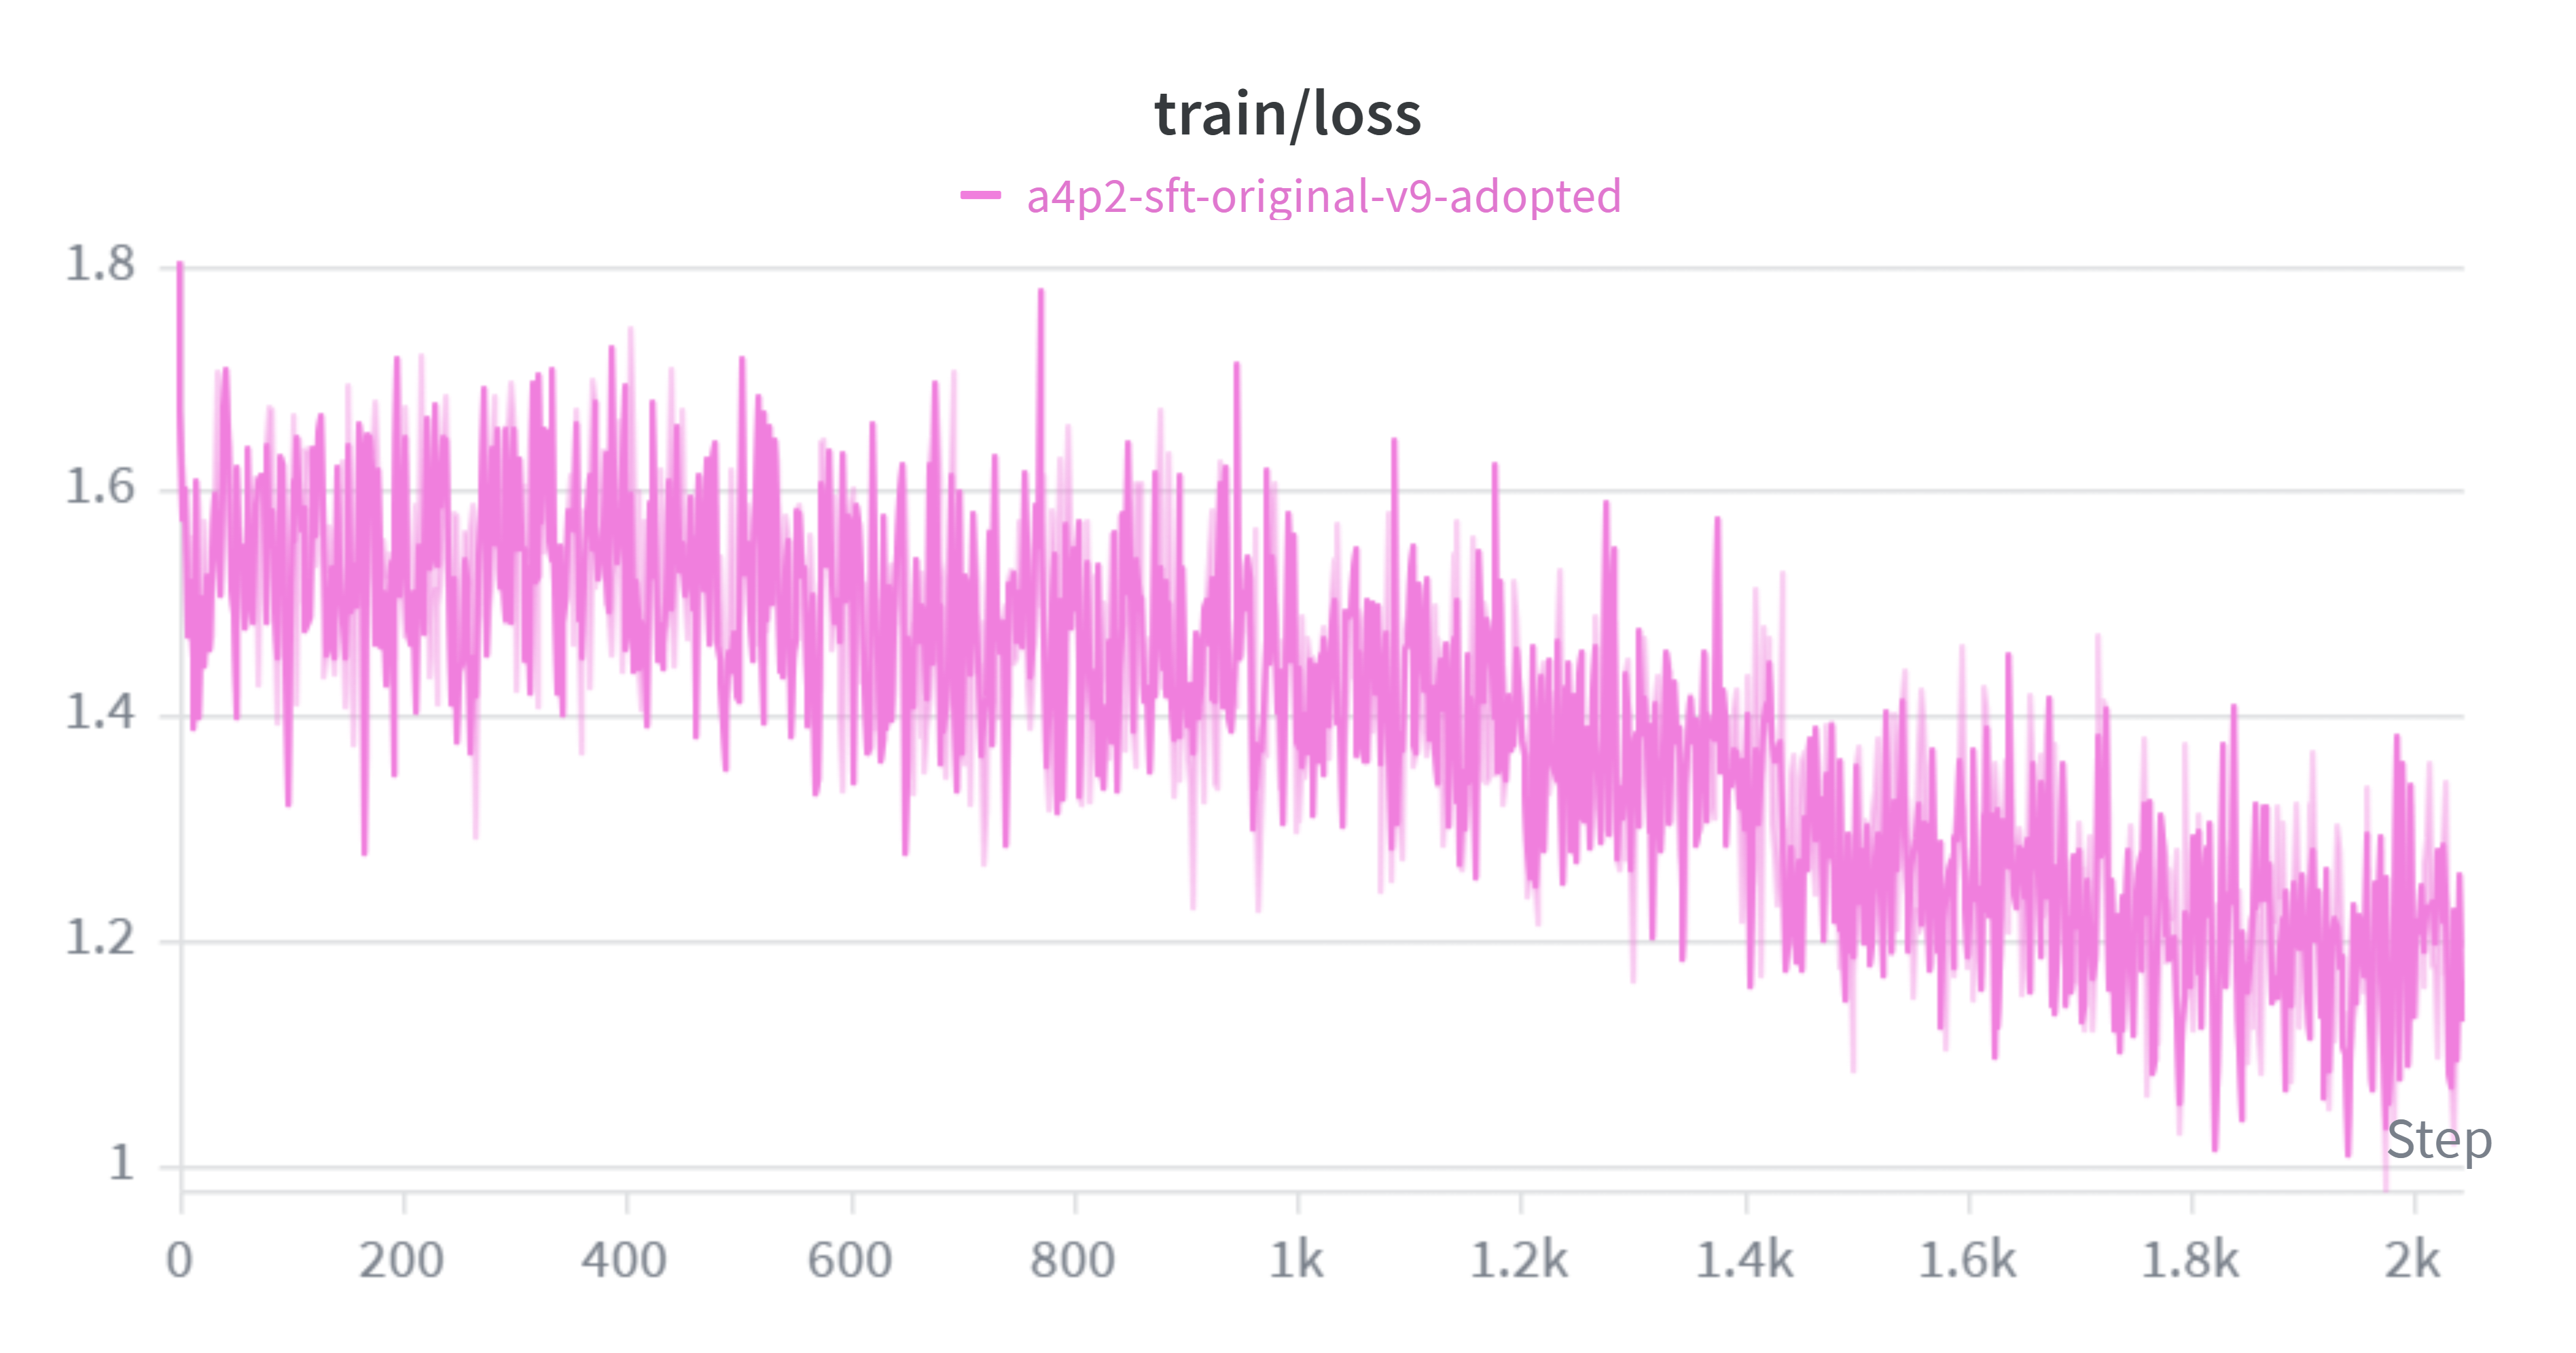
\includegraphics[width=0.8\linewidth]{component/figures/p2/sft_loss.png }
    \caption{Training loss for the original-configuration SFT run logged in Weights \& Biases. 
    The loss decreases steadily from approximately 1.6 to around 1.2 over the training steps, 
    indicating stable optimization under the supervised fine-tuning objective. The high 
    variance between steps is expected due to small per-device batch sizes and stochastic 
    sampling of instruction-style training data.}
    \label{fig:sft_loss}
\end{figure}

\begin{figure}[H]
    \centering
    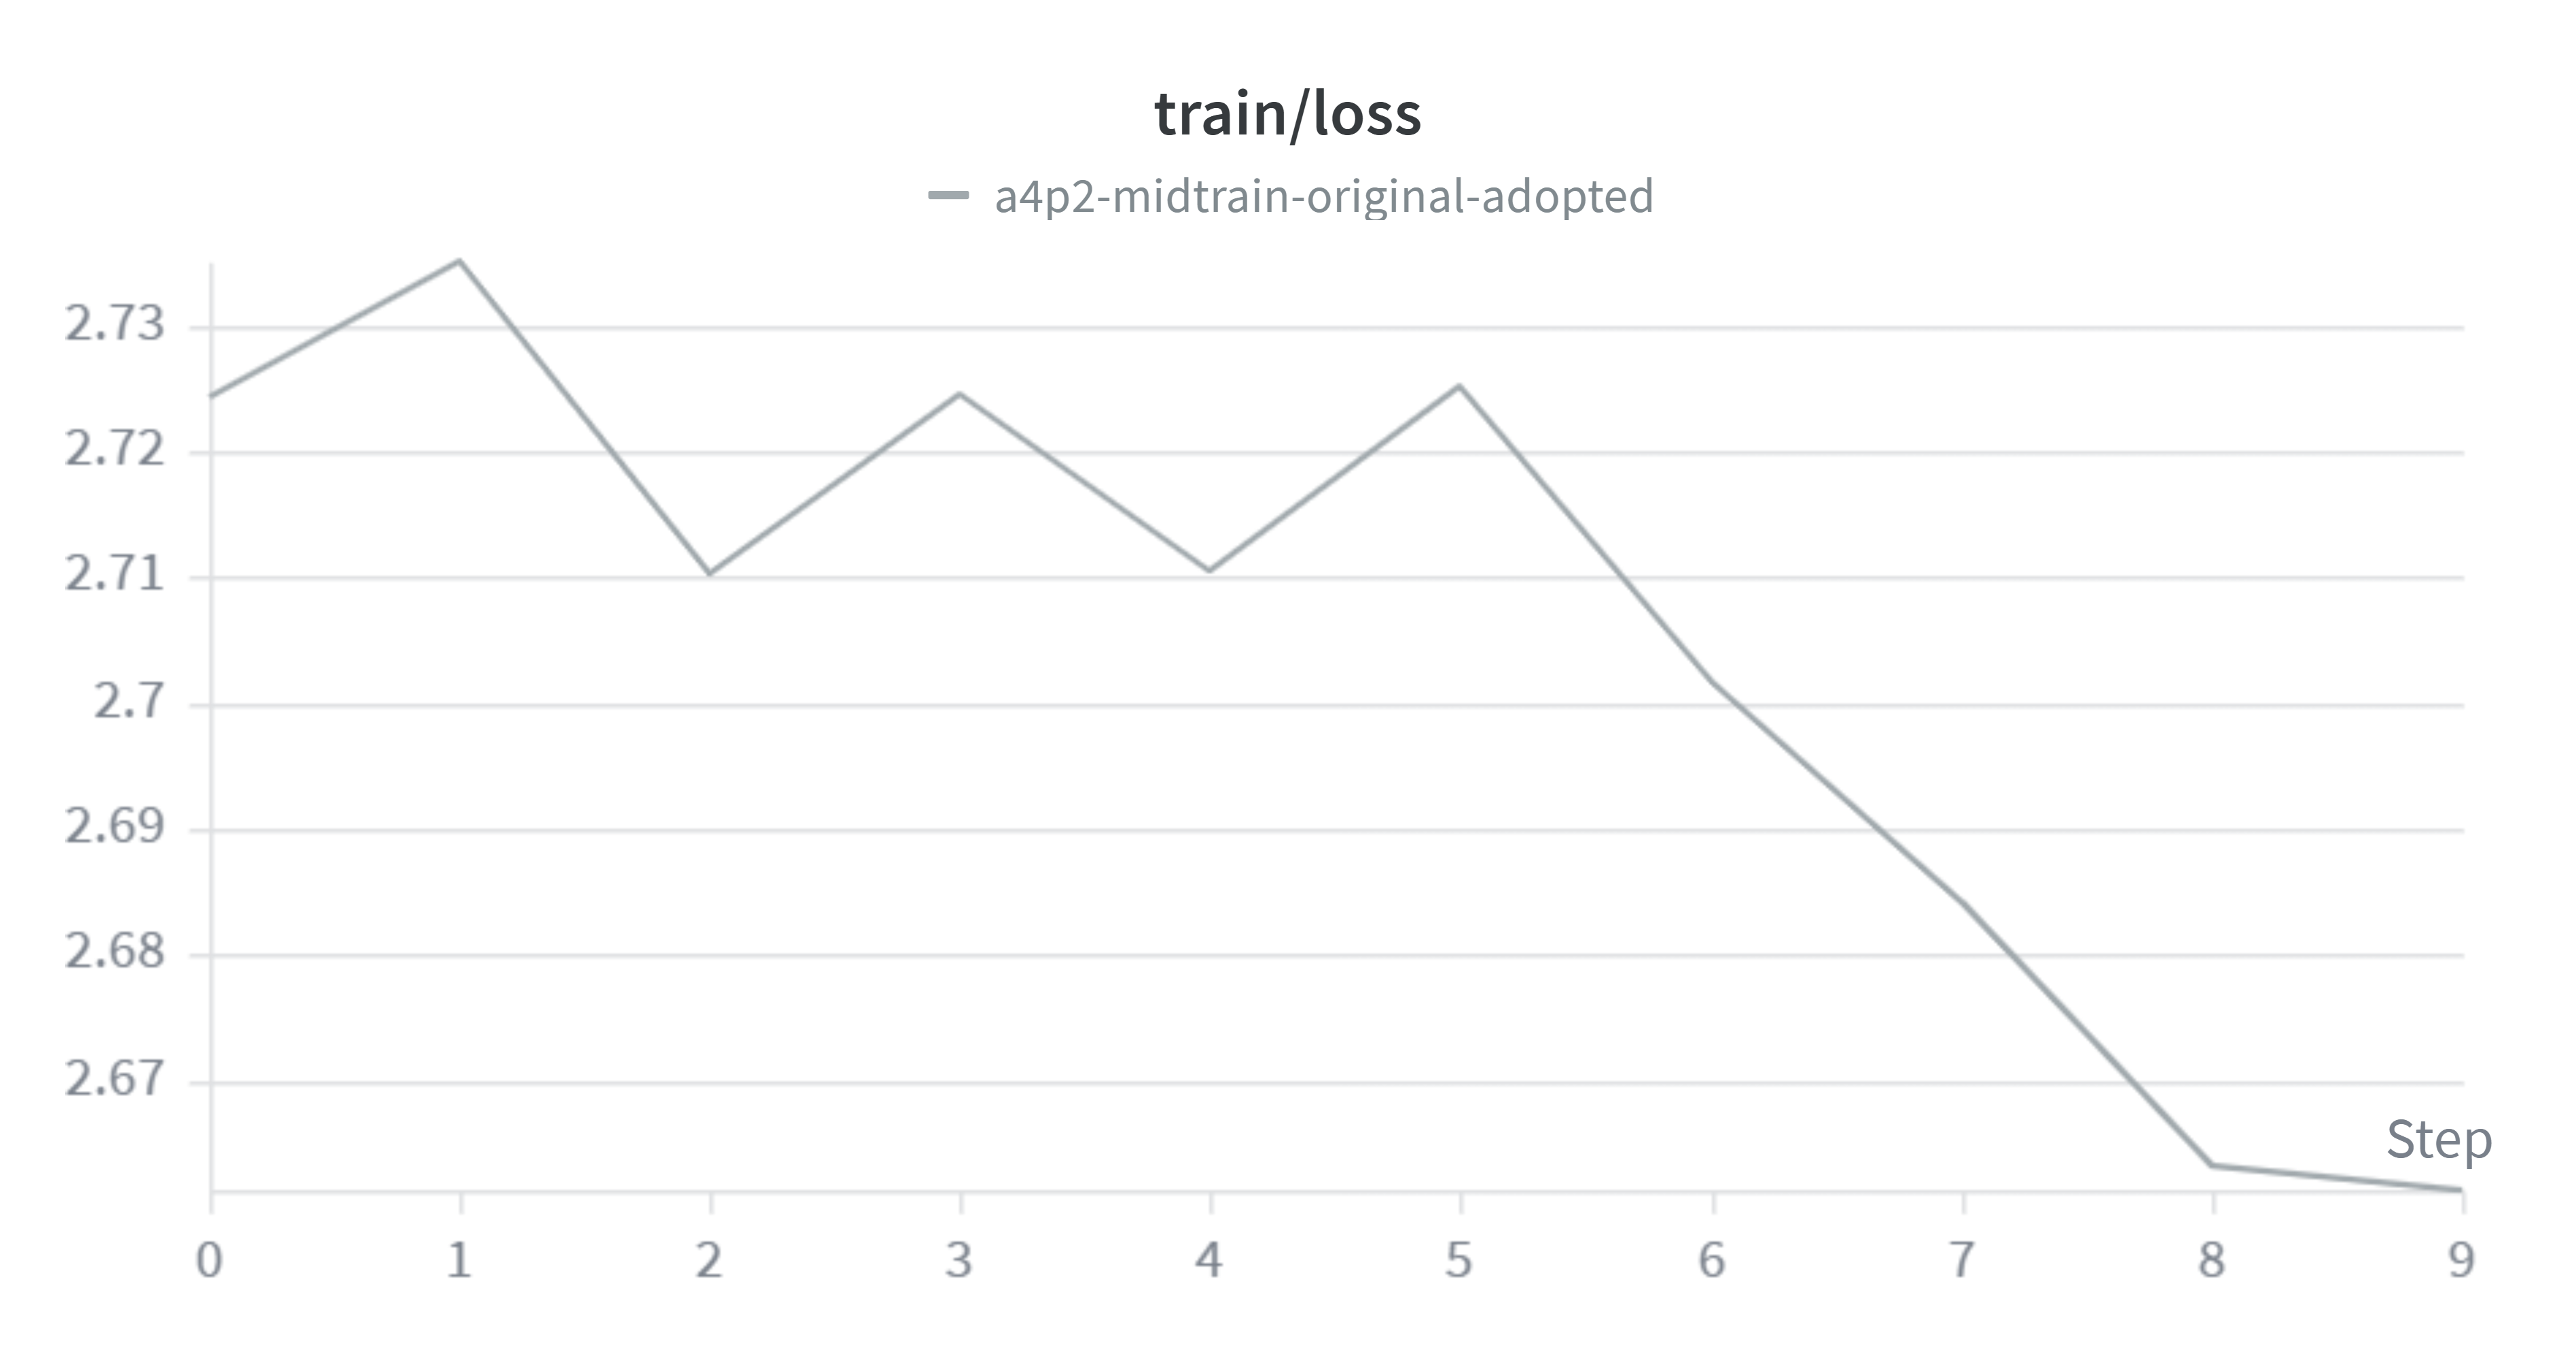
\includegraphics[width=0.8\linewidth]{component/figures/p2/midtrain_loss.png}
    \caption{Training loss for the original-configuration midtraining run. 
    Although the number of logged steps is smaller, the loss trend shows a gradual 
    reduction across steps, suggesting the model continues to optimize the 
    language-modeling objective during additional token training.}
    \label{fig:midtrain_loss}
\end{figure}

\begin{figure}[H]
    \centering
    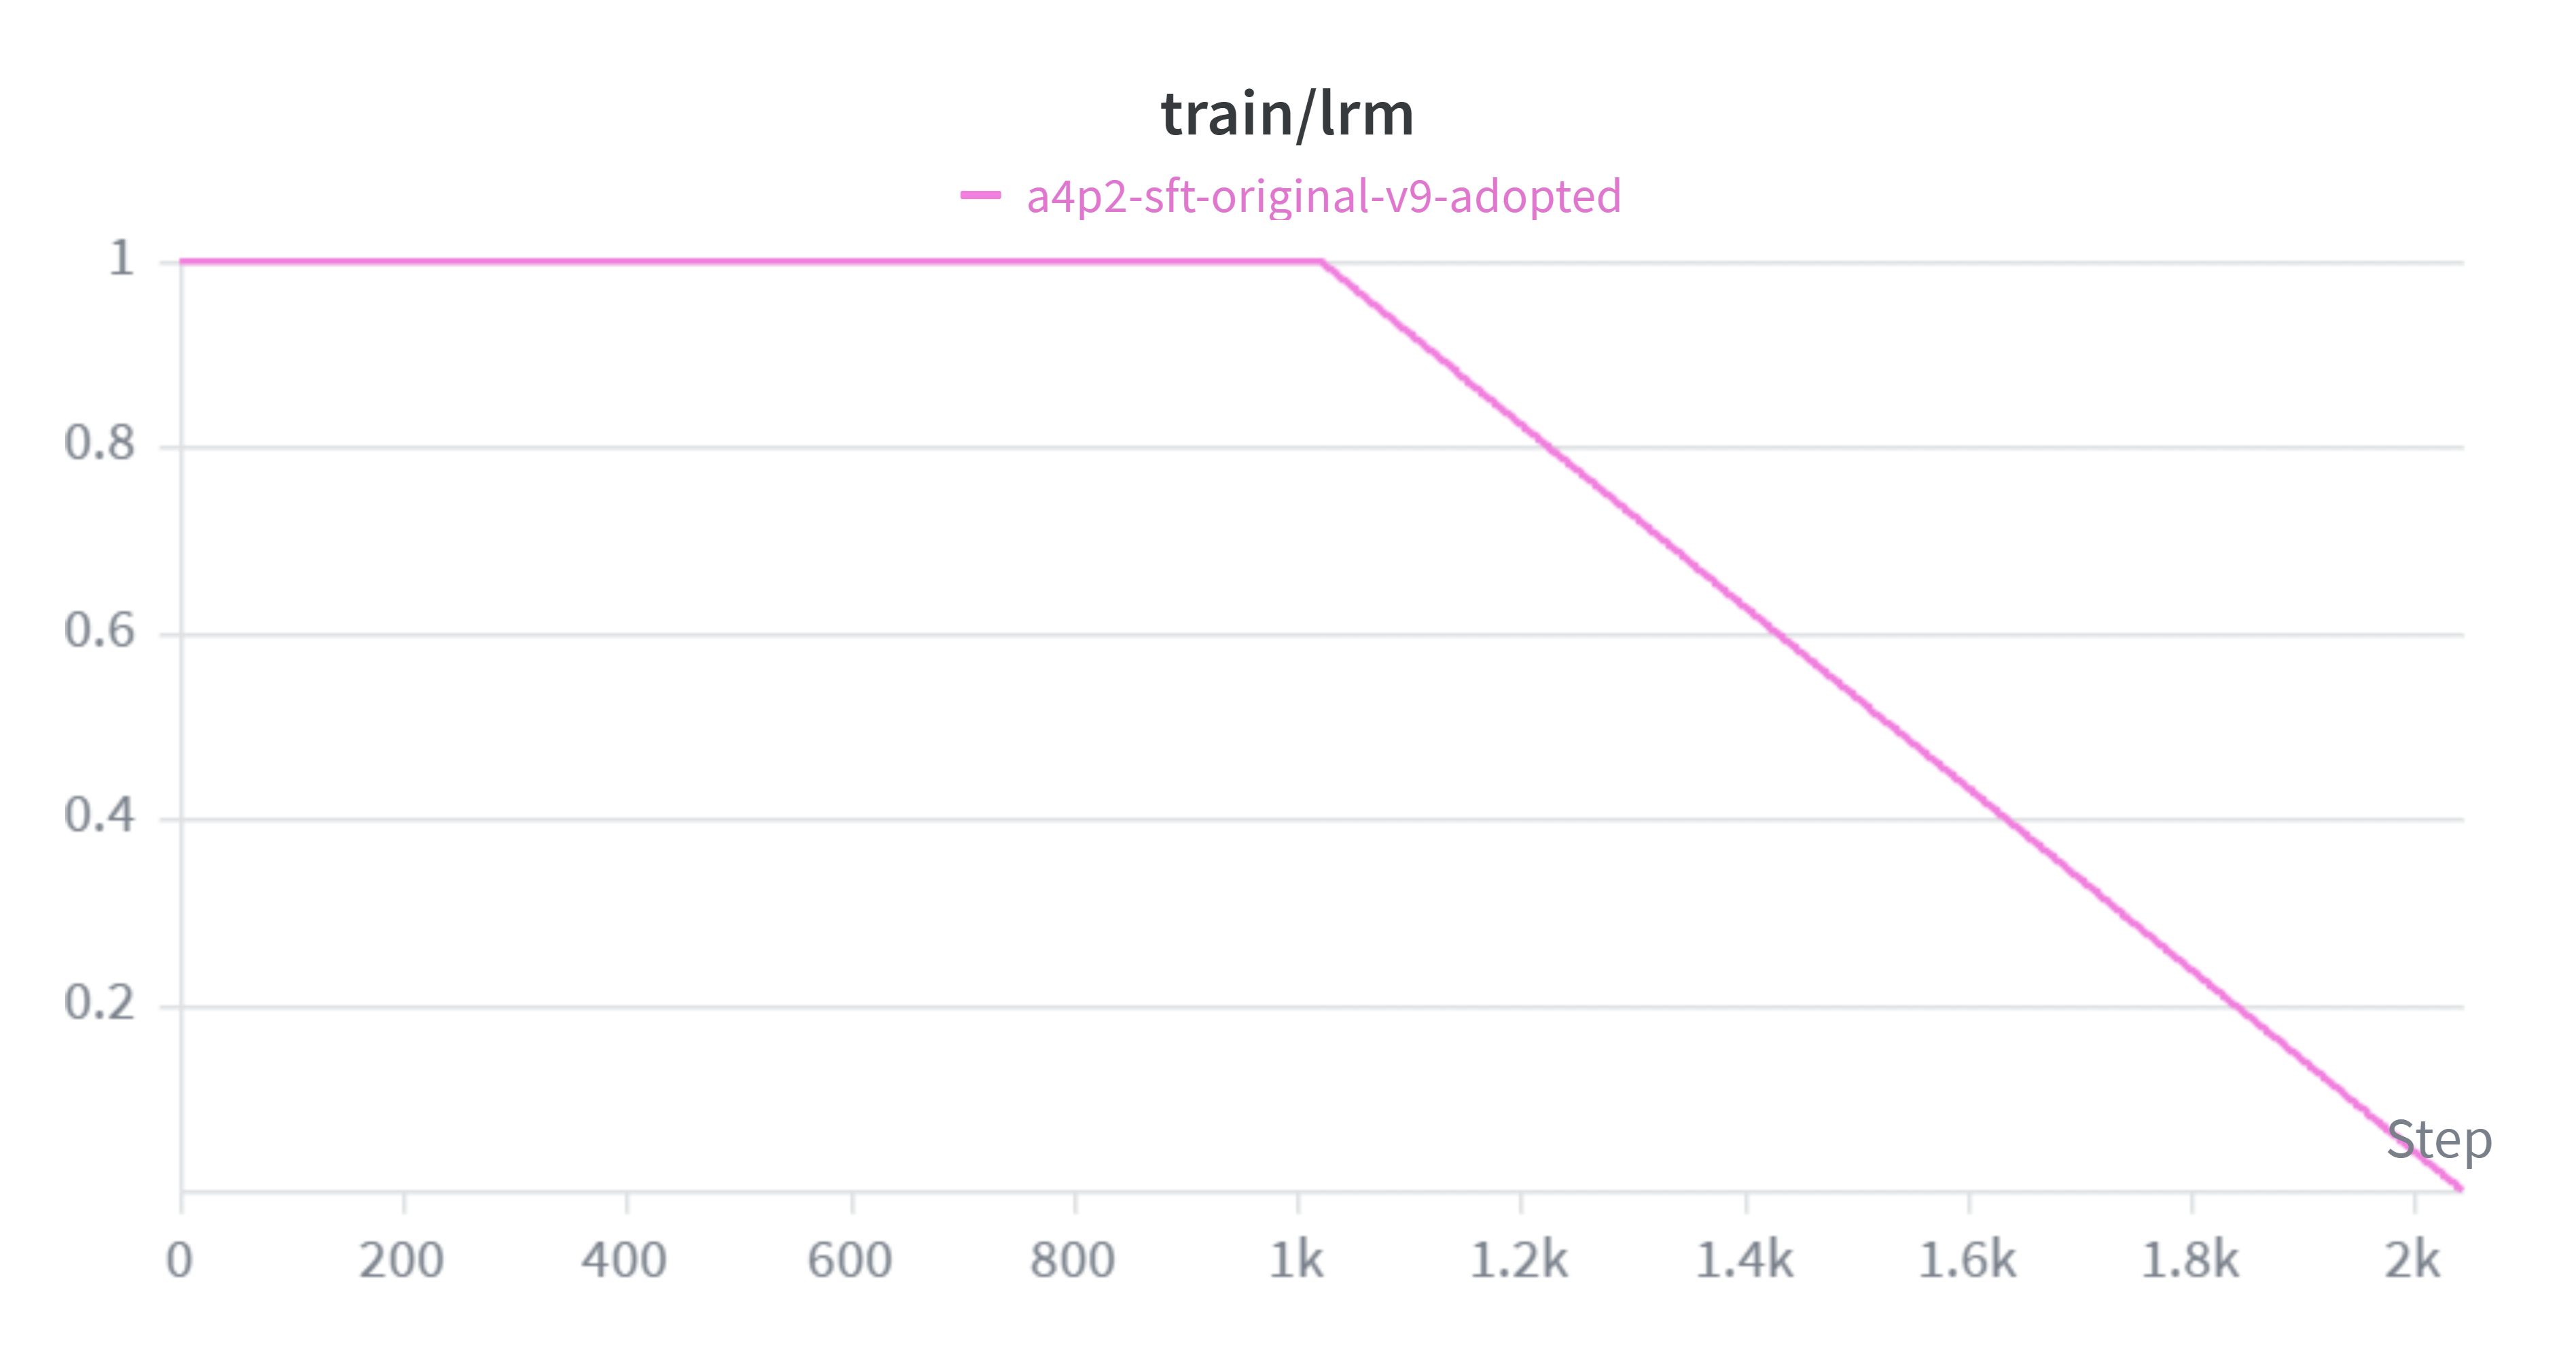
\includegraphics[width=0.8\linewidth]{component/figures/p2/sft_lr.png}
    \caption{Learning-rate multiplier schedule used during SFT. The learning rate 
    remains constant during the initial training phase and then linearly decays, 
    following the scheduler configuration in the original SFT script.}
    \label{fig:sft_lrm}
\end{figure}
\begin{figure}[H]
    \centering
    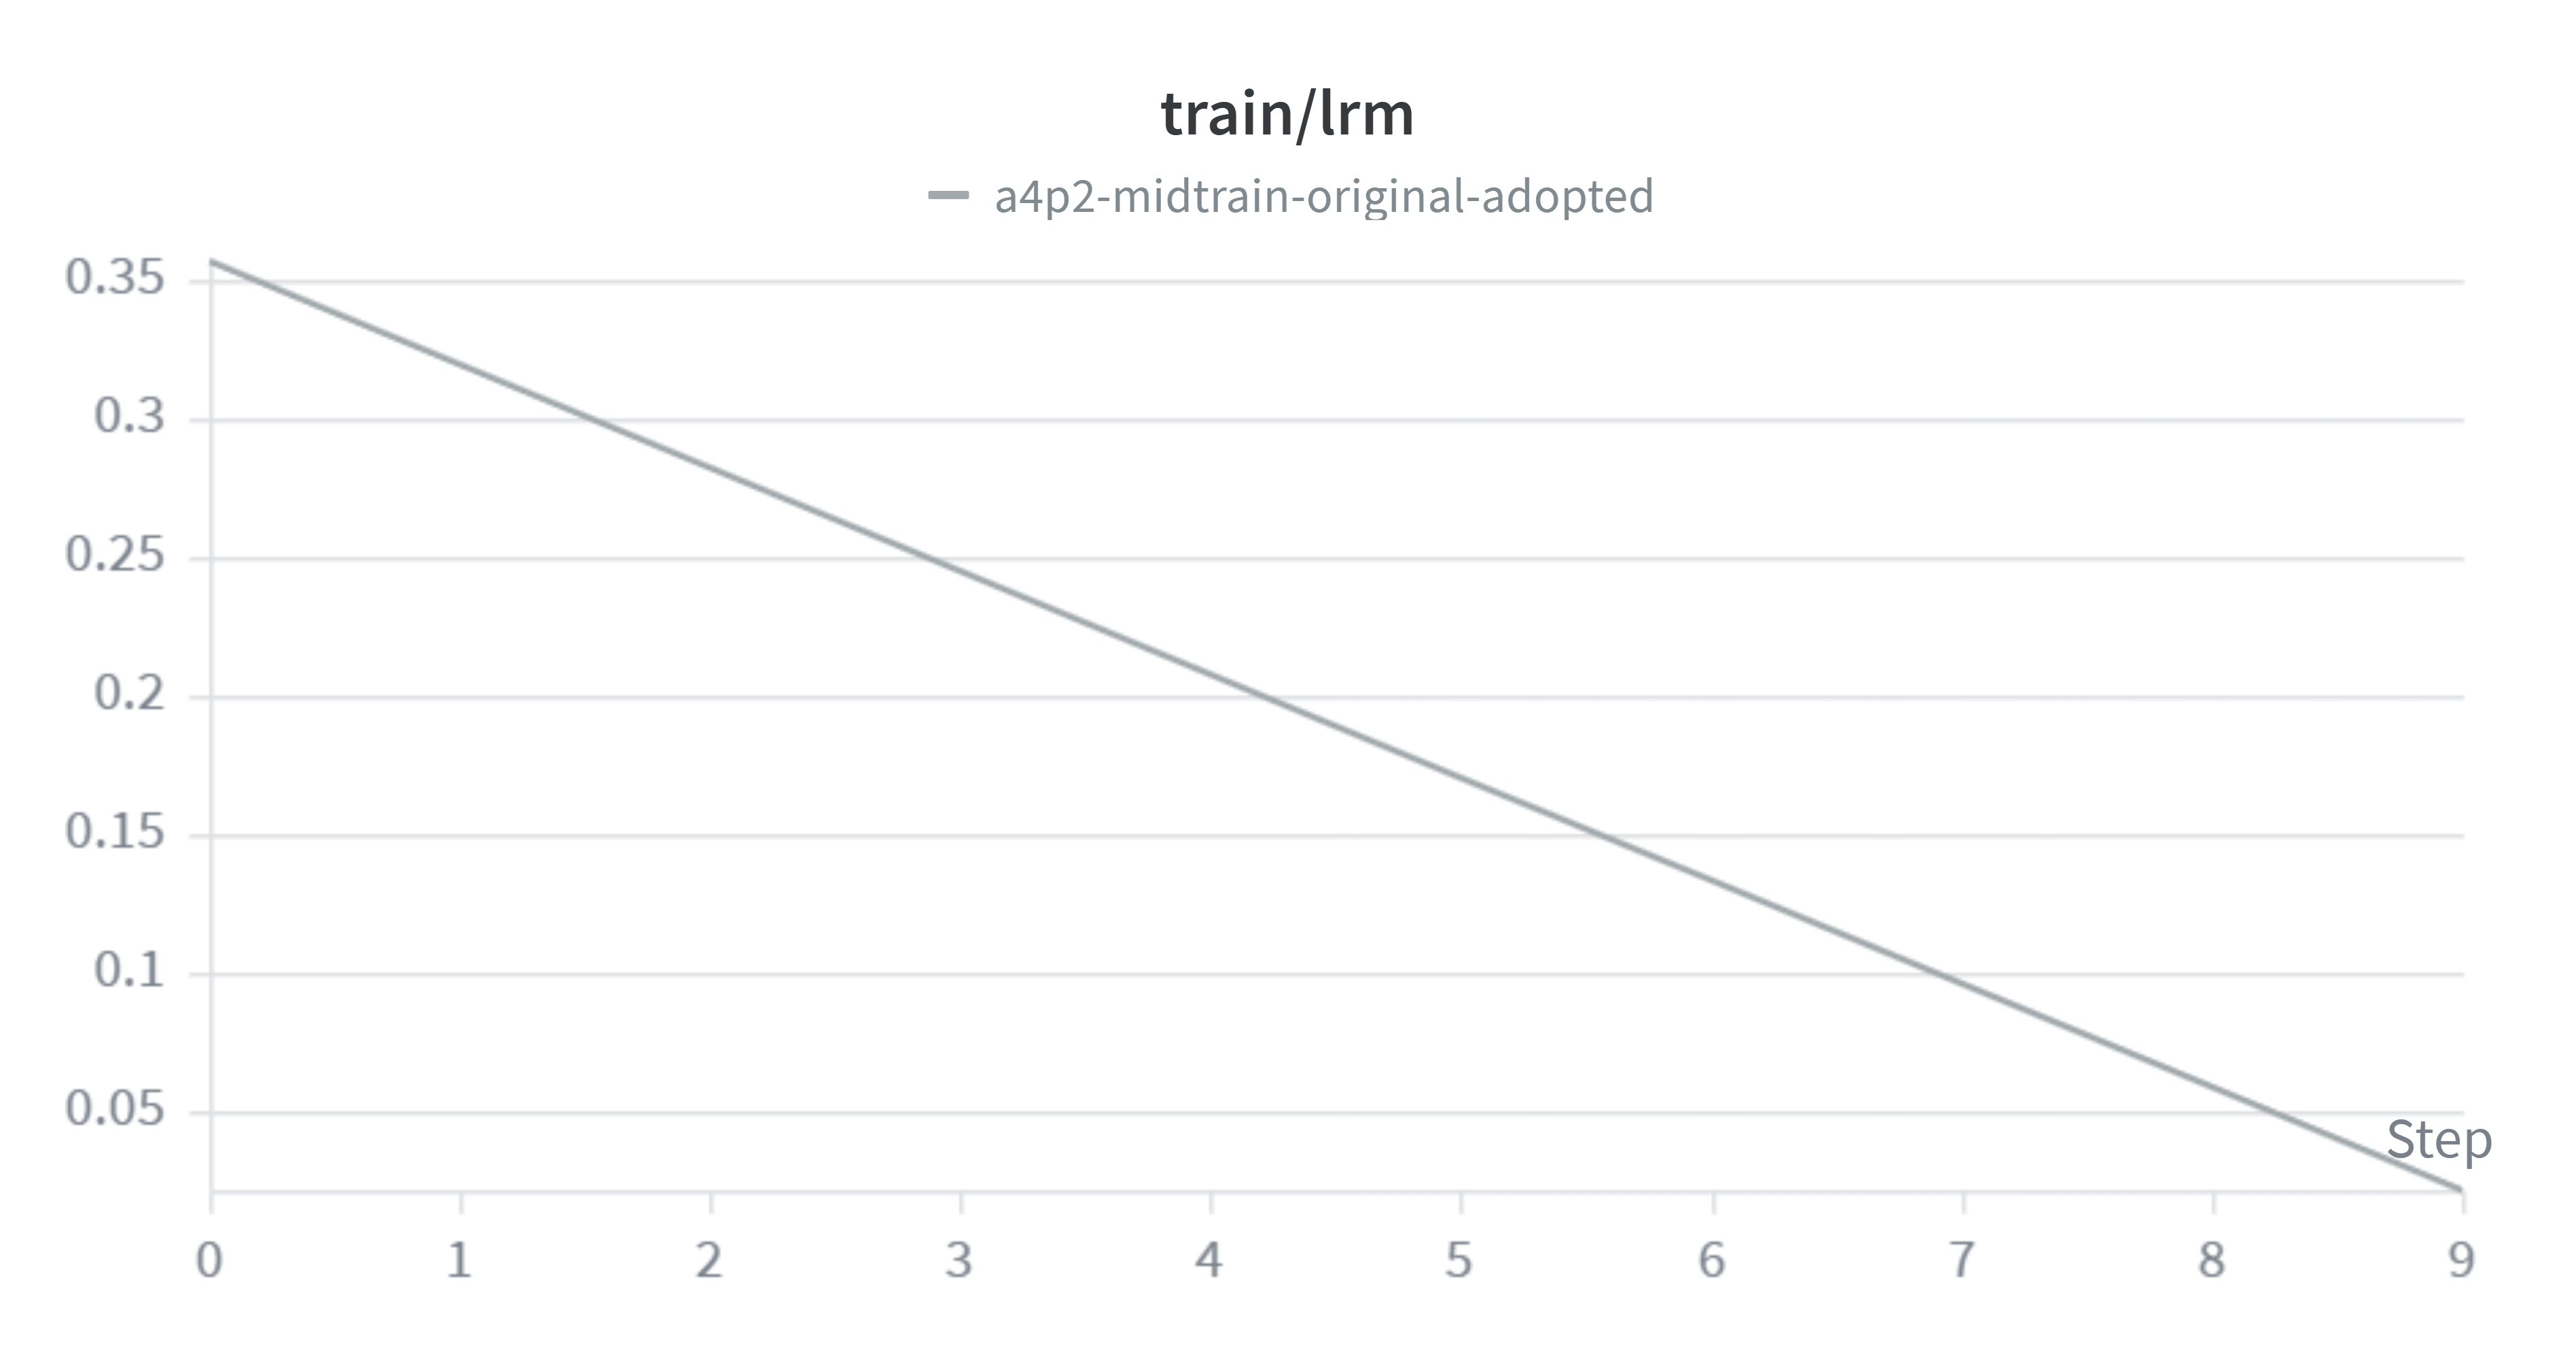
\includegraphics[width=0.8\linewidth]{component/figures/p2/midtrain_lr.png}
    \caption{Learning-rate multiplier schedule for the midtraining run, showing the 
    expected linear decay over training steps according to the original configuration.}
    \label{fig:midtrain_lrm}
\end{figure}
\paragraph{Discussion.}
Overall, the original-configuration ablation produces a clear ranking for this task: SFT is the only stage that materially improves GSM8K performance over the pretrained baseline, while midtraining alone does not. The evidence suggests that, for this checkpoint and evaluation setup, instruction- or response-format adaptation is more important than further generic language-model optimization when the downstream target is grade-school math reasoning. Put differently, SFT improves \emph{how} the model answers, and that change is what yields the measurable GSM8K gain.

At the same time, the SFT result should not be overstated. Even after SFT, strict accuracy is only 5.23\%, so the model is still weak at robust mathematical reasoning. The main benefit of this stage is that it converts an almost entirely unscorable model into one that often produces structured, parseable, and occasionally correct numeric solutions. This makes SFT a strong precursor stage for later RL-based improvement, because RL can only effectively reinforce behaviors that are already appearing with non-trivial frequency.

\paragraph{Conclusion.}
For Part 2's original-configuration comparison, the main conclusion is that SFT provides the only meaningful downstream benefit on GSM8K. Midtraining slightly improves the language-modeling objective but fails to improve answer formatting or math accuracy. Therefore, under the original scripts, SFT is the more effective adaptation stage for preparing the pretrained nanochat checkpoint for subsequent task-focused optimization.


\paragraph{GSM8K Evaluation Definitions}
\label{sec:gsm8k_eval_def}

Strict accuracy requires the model’s final answer to be recoverable by the standard GSM8K
answer extractor and to exactly match the reference extracted answer. Relaxed accuracy
allows a fallback heuristic: if the standard extractor fails, the evaluator uses the last
numeric value appearing in the response and counts it as correct if it is numerically equal
to the gold answer.



\subsection{Additional Dataset Experiments}

To explore whether domain-specific data improves mathematical reasoning, we performed
additional SFT and midtraining runs using external datasets while keeping all training
hyperparameters identical to the original configurations. This isolates the effect of the
training data itself and avoids introducing confounding hyperparameter changes.

\subsubsection{Datasets}

Two additional datasets were selected to augment the training process:

\begin{itemize}
\item \textbf{MetaMathQA (50k subset)} for SFT.  
MetaMathQA contains structured mathematical reasoning examples and step-by-step
solutions, making it suitable for supervised instruction tuning. The dataset format
matches conversational math explanations, which aligns well with the chat-style
fine-tuning objective.

\item \textbf{FineMath 4+ Mix} for midtraining.  
FineMath is a curated corpus of high-quality mathematical text and problem-solving
content. Using this dataset during midtraining exposes the base model to a large amount
of mathematical language and reasoning patterns before downstream evaluation.
\end{itemize}

The SFT run incorporated the MetaMathQA dataset as additional conversations in JSONL
format, while the midtraining run replaced the default training corpus with the
FineMath mixture directory.

\subsubsection{Training Configuration}

To ensure a fair comparison, the additional dataset runs used exactly the same
hyperparameters as the original training procedures.

\begin{table}[h]
\centering
\small
\begin{tabular}{l l l}
\hline
\textbf{Parameter} & \textbf{Value} & \textbf{Purpose} \\
\hline
device\_batch\_size & 8 (SFT), 32 (midtraining) & Maintain original memory footprint \\
total\_batch\_size & 16384 (SFT), 1048576 (midtraining) & Preserve effective batch scaling \\
attention\_impl & fa3 & Efficient FlashAttention implementation \\
max\_seq\_len & 512 & Match base training context length \\
depth & 20 (midtraining) & Same architecture as base model \\
mlp\_variant & SwiGLU & Same MLP structure used in base model \\
residual\_variant & standard & Preserve architecture behavior \\
fp8 training & enabled (midtraining) & Maintain original efficiency setup \\
render\_max\_tokens & 513 & Same decoding configuration for SFT \\
\hline
\end{tabular}
\caption{Training configuration used for additional dataset experiments.}
\end{table}

The MetaMath SFT run used the same chat fine-tuning script with an additional JSONL
conversation file containing MetaMathQA examples
(\texttt{metamathqa\_50k.jsonl}) 
Similarly, the midtraining run used the same base training script but pointed the
training data directory to the FineMath dataset
(\texttt{finemath\_4plus\_mix}) 

\subsubsection{Training Behaviour}

Figures~\ref{fig:sft_loss_compare}--\ref{fig:midtrain_lr_compare} summarize the training
dynamics observed in Weights \& Biases for both the original and additional dataset runs.
For each training stage we report the training loss and learning-rate schedule.

\begin{figure}[h]
\centering
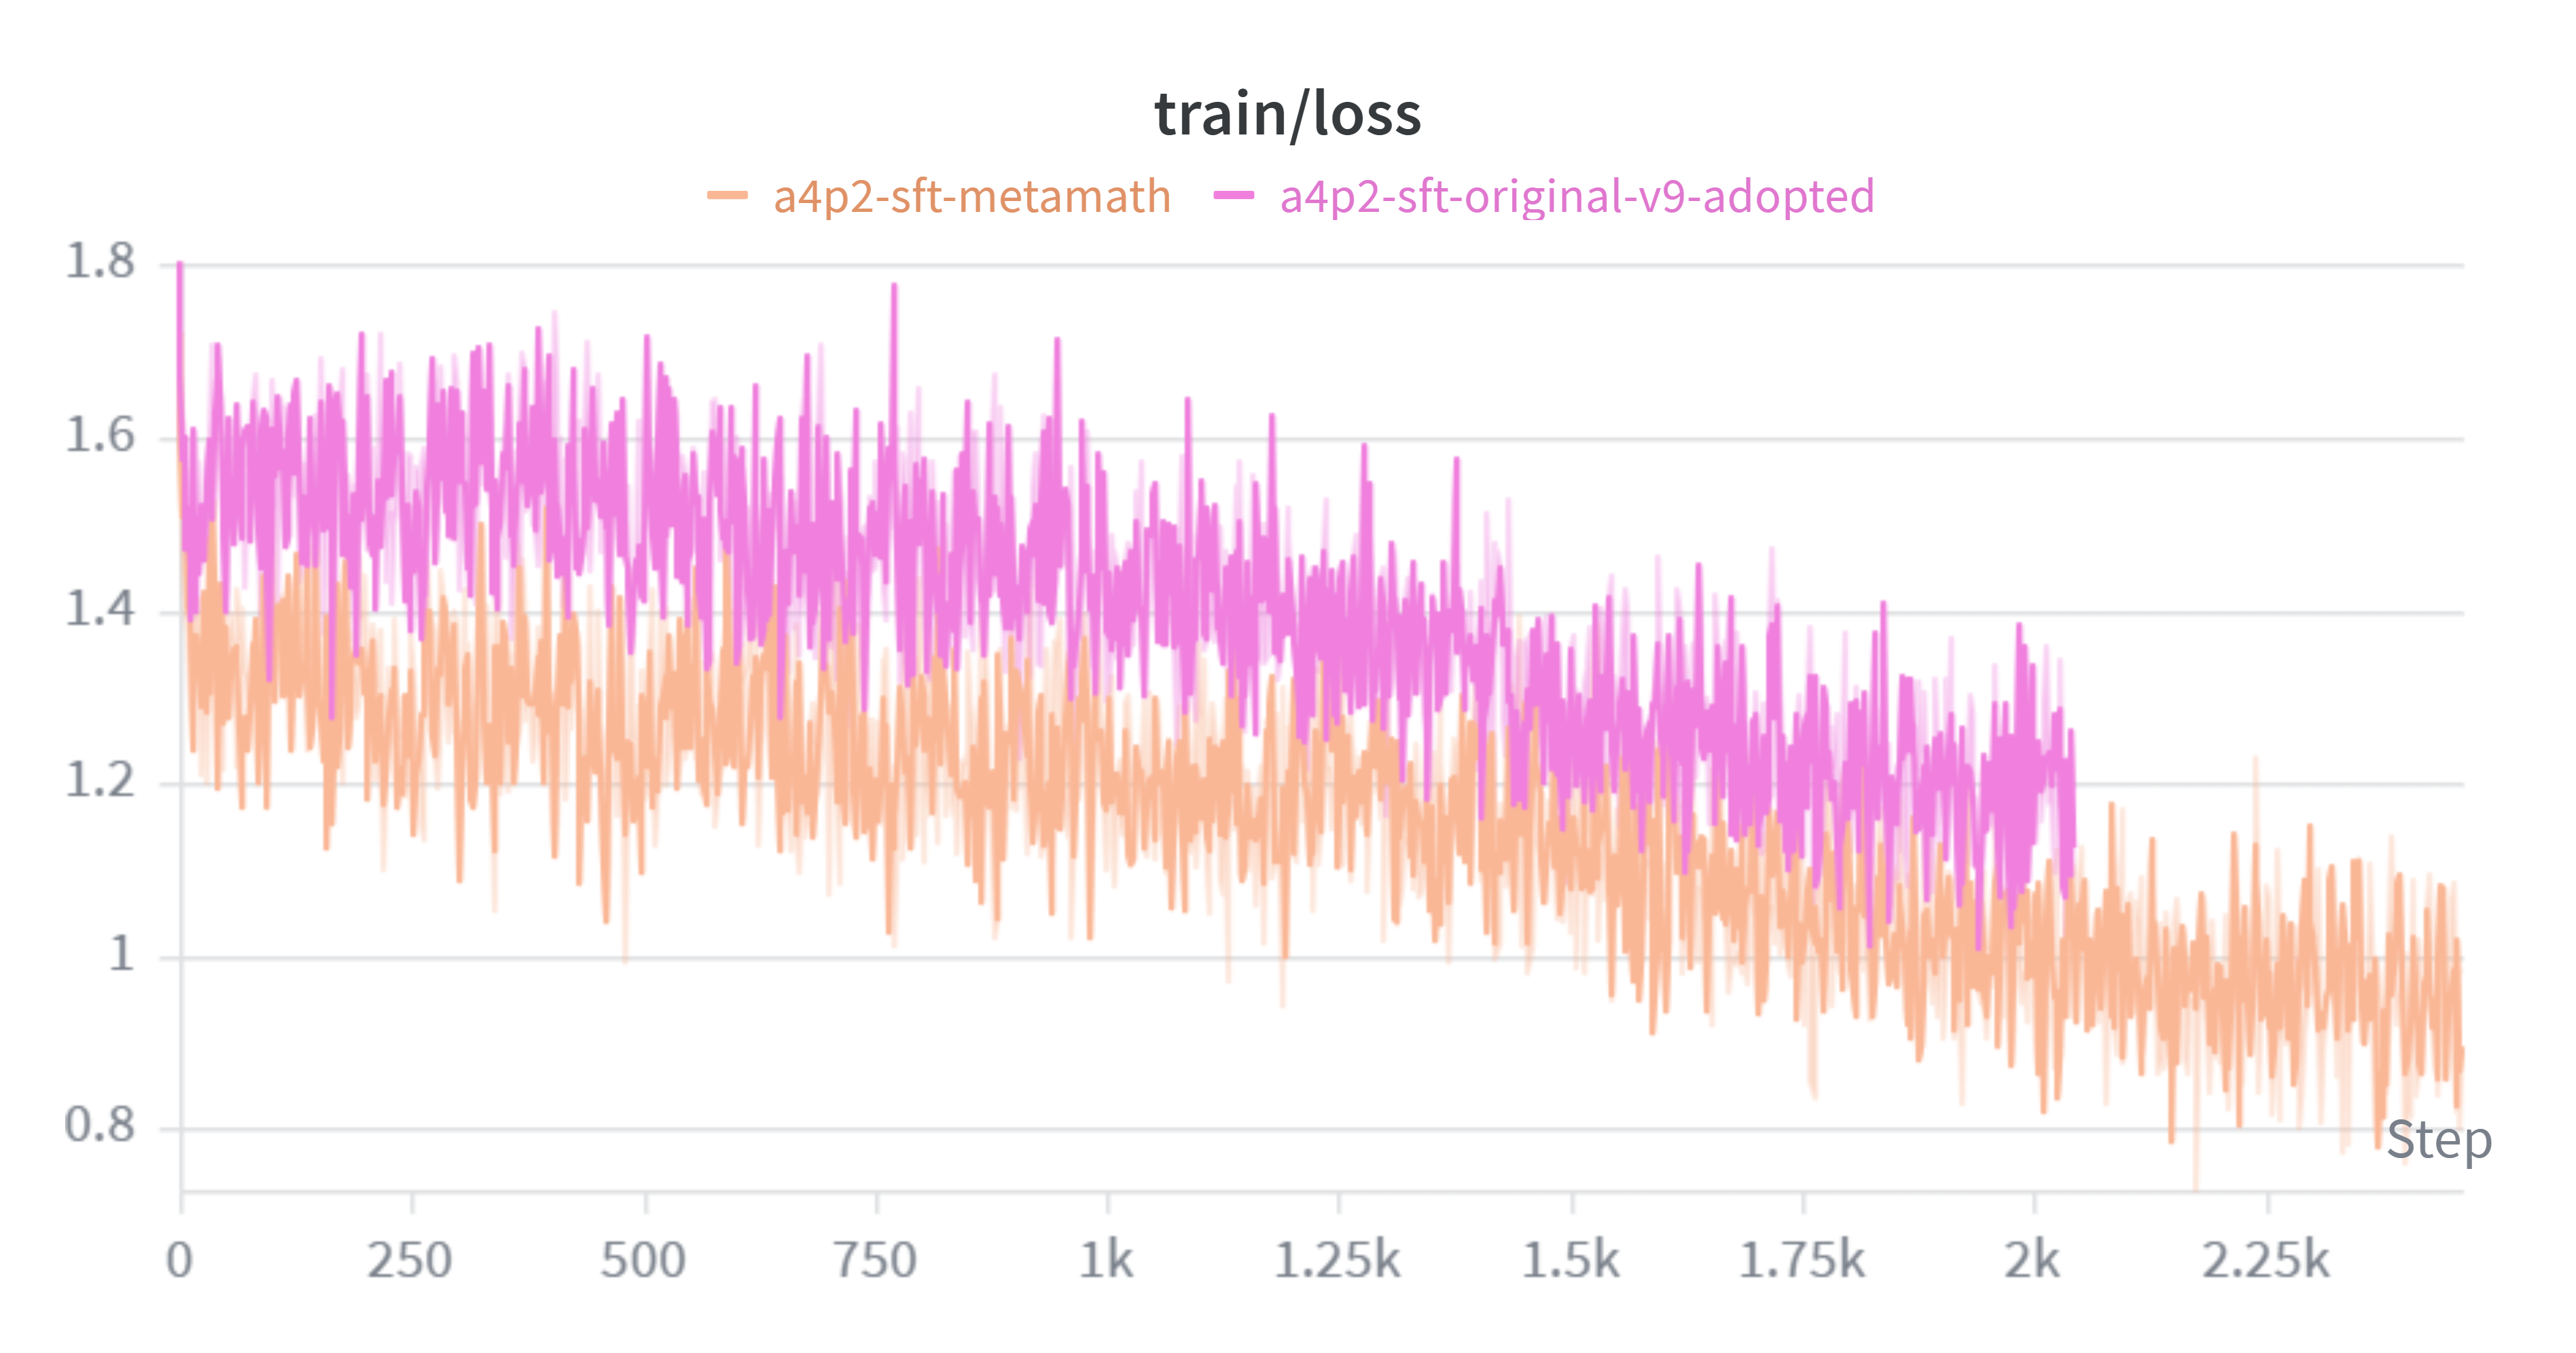
\includegraphics[width=0.75\linewidth]{component/figures/p2/meta_sft_loss.png}
\caption{Training loss comparison between the original SFT run and the MetaMath SFT run.}
\label{fig:sft_loss_compare}
\end{figure}

\begin{figure}[h]
\centering
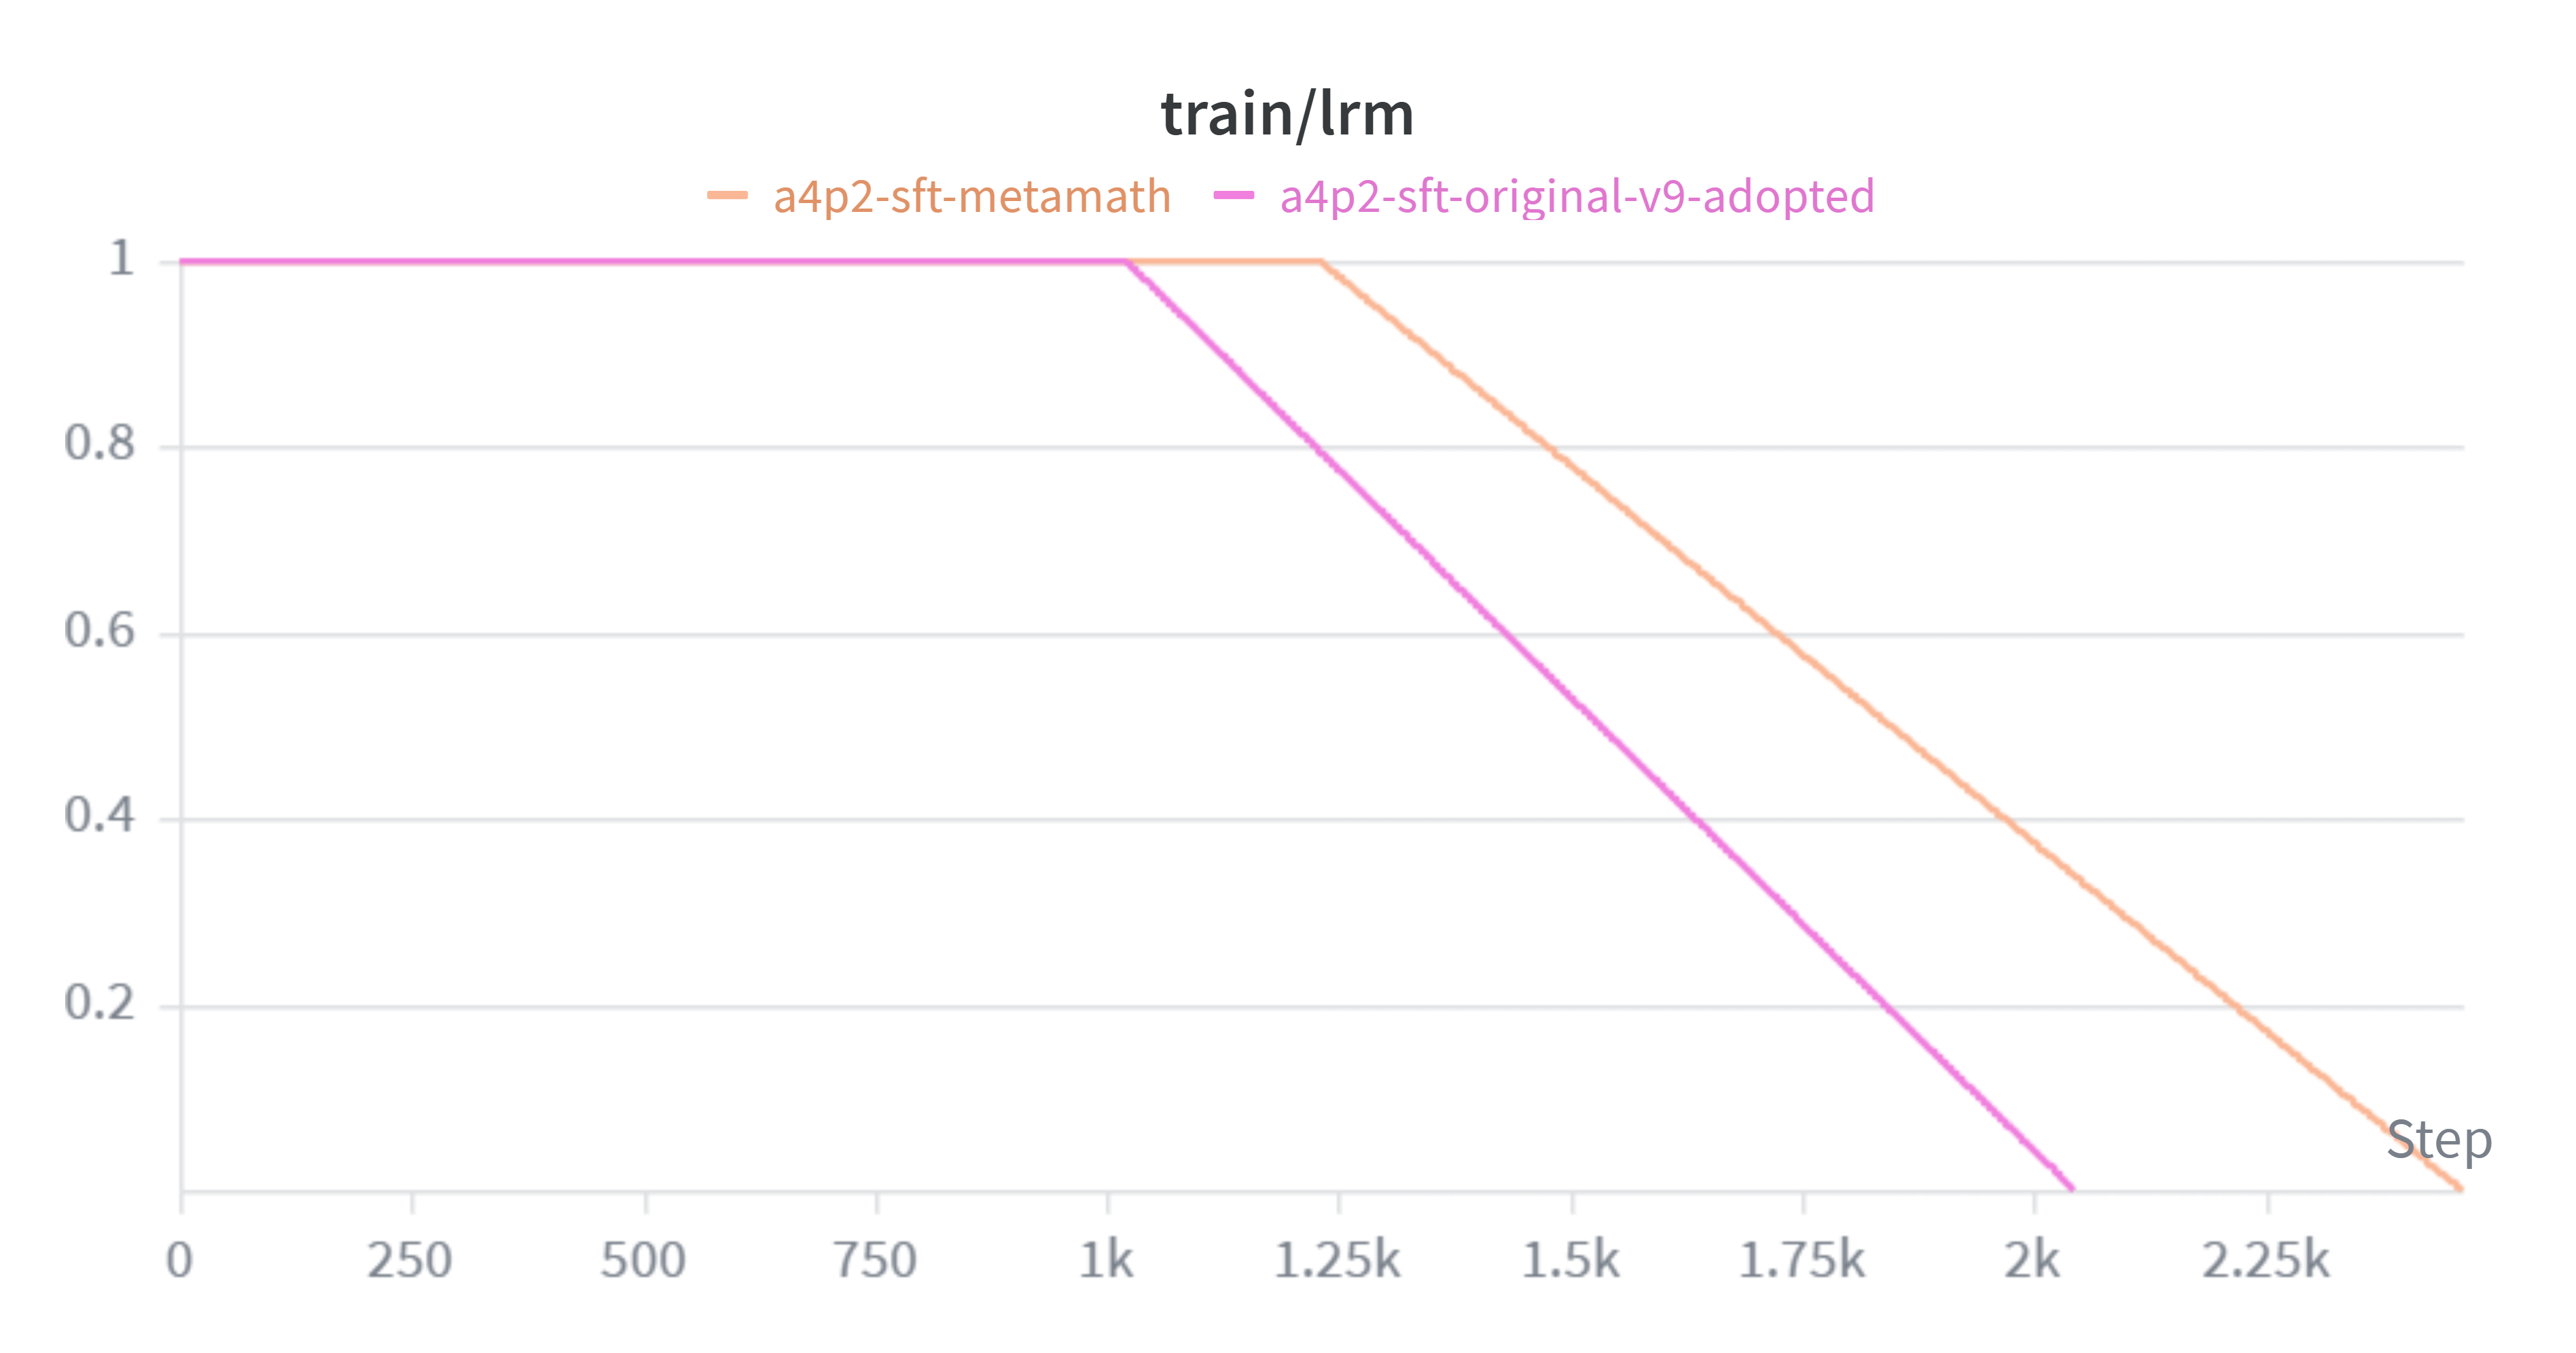
\includegraphics[width=0.75\linewidth]{component/figures/p2/meta_sft_lr.png}
\caption{Learning rate schedule during SFT for the original and MetaMath runs.}
\label{fig:sft_lr_compare}
\end{figure}

\begin{figure}[h]
\centering
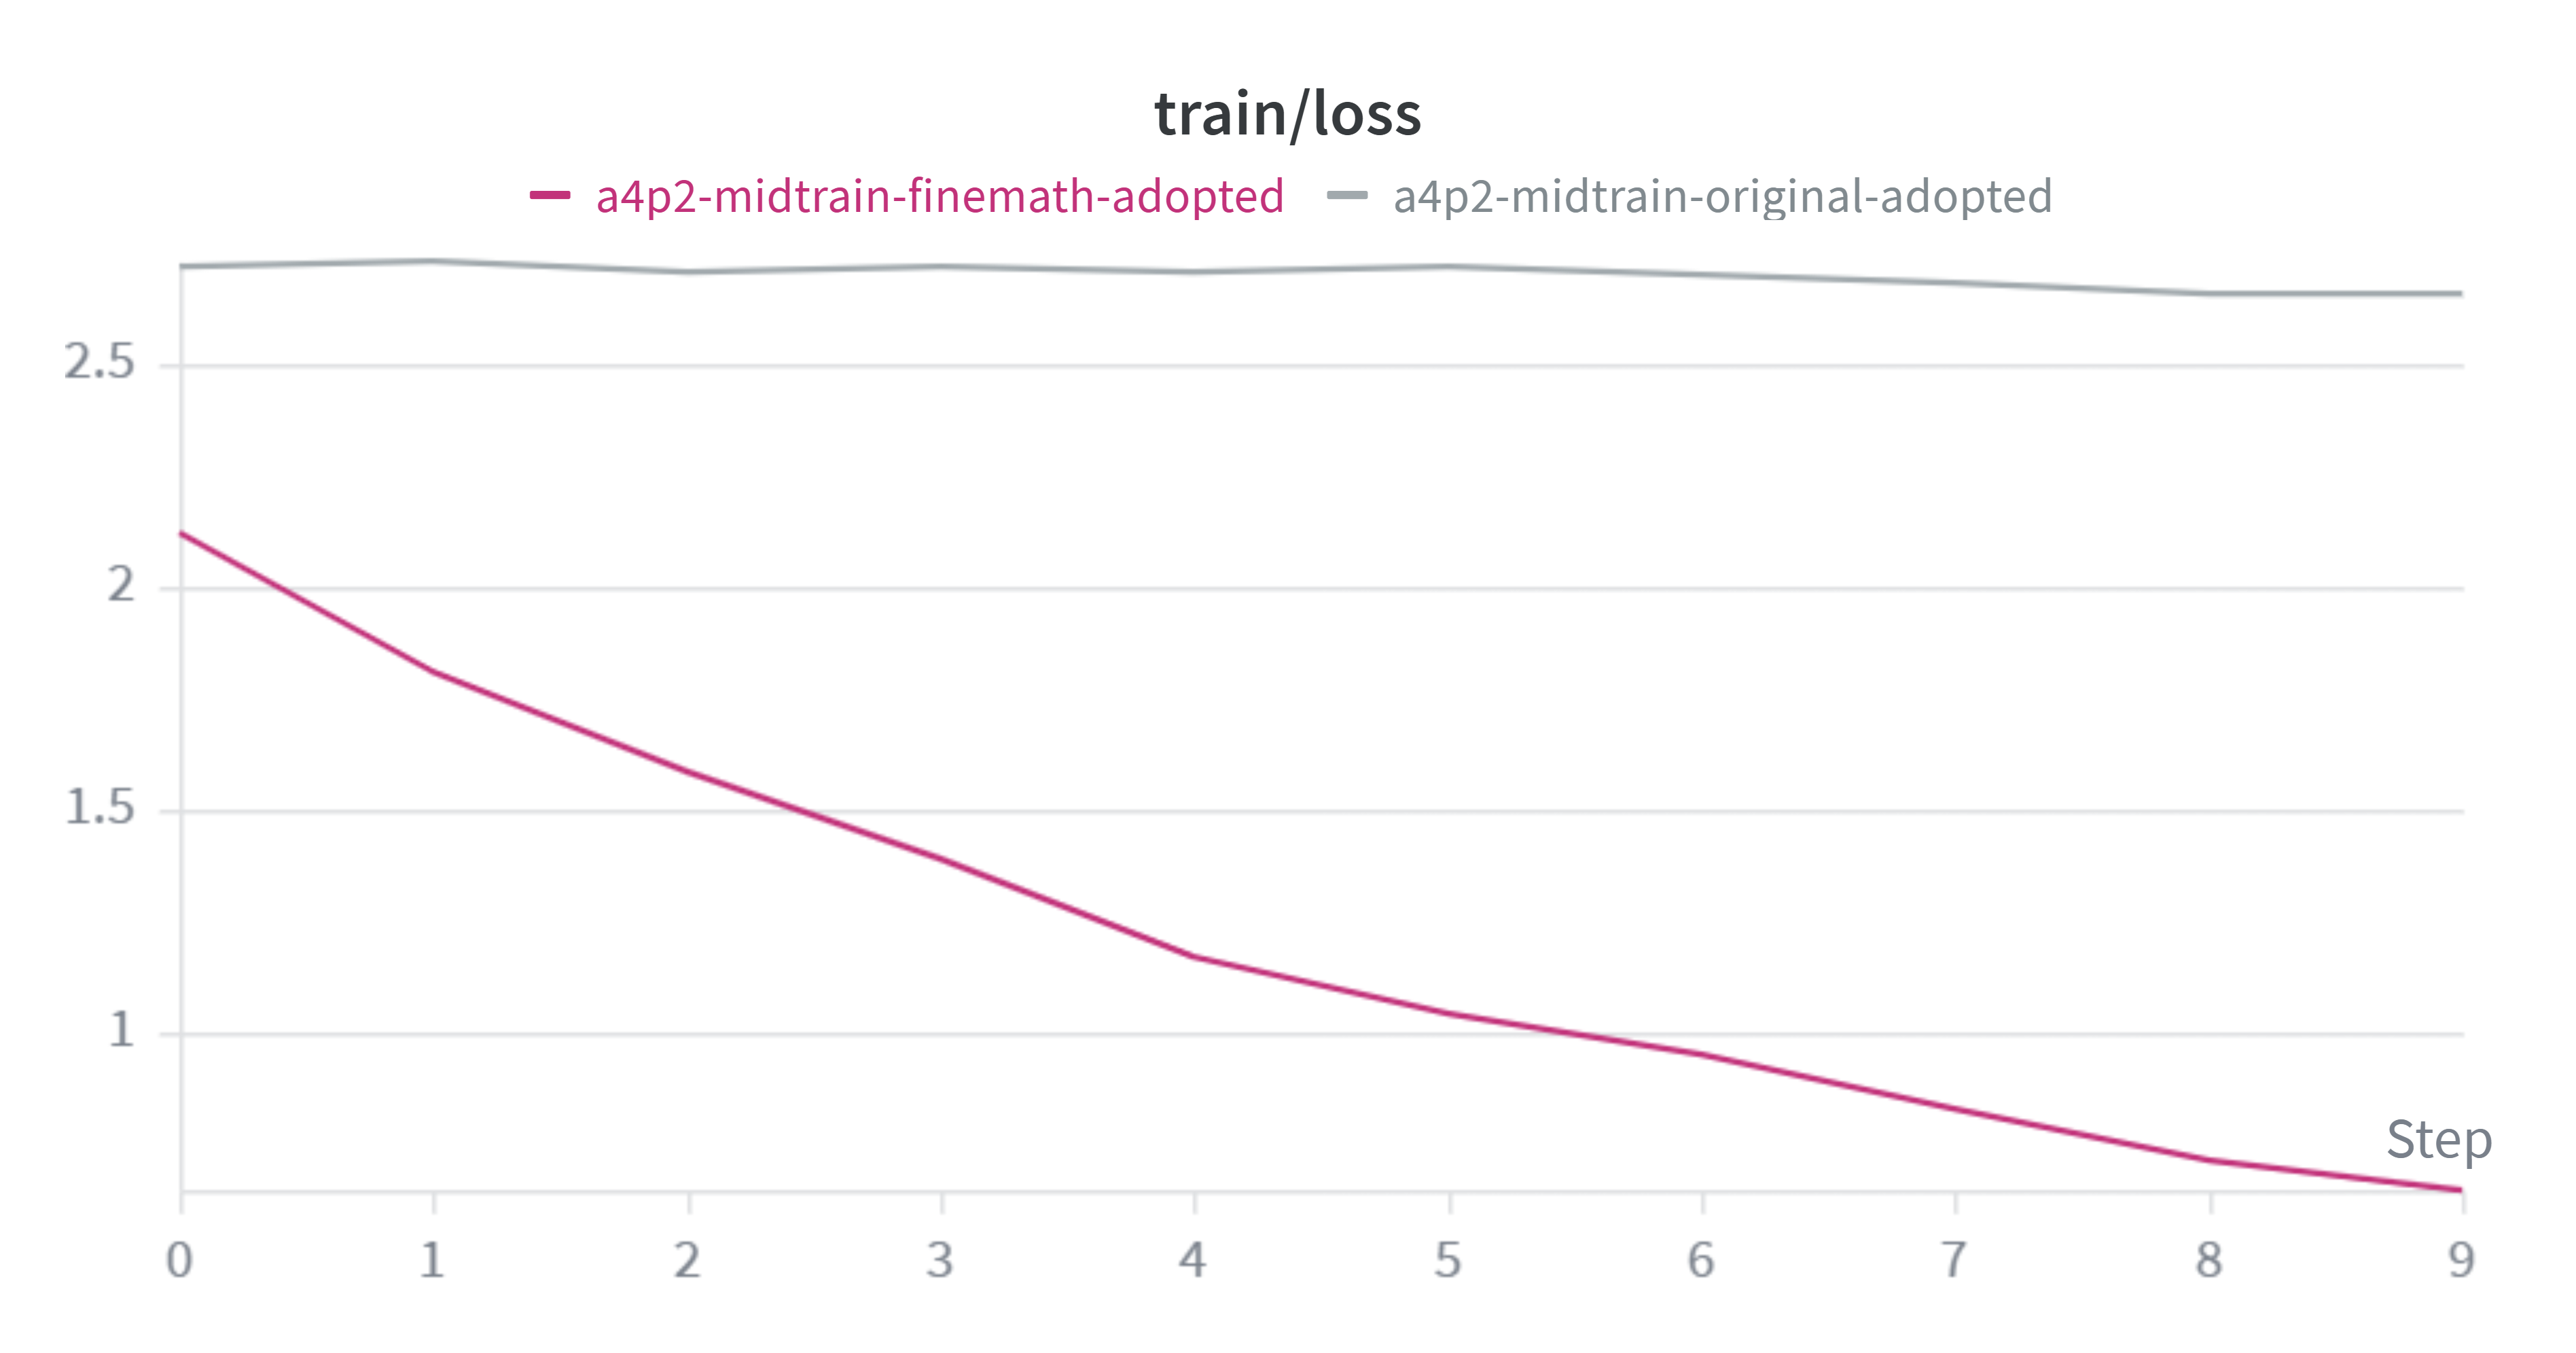
\includegraphics[width=0.75\linewidth]{component/figures/p2/midtrain_math_loss.png}
\caption{Training loss comparison between the original midtraining run and the FineMath midtraining run.}
\label{fig:midtrain_loss_compare}
\end{figure}

\begin{figure}[h]
\centering
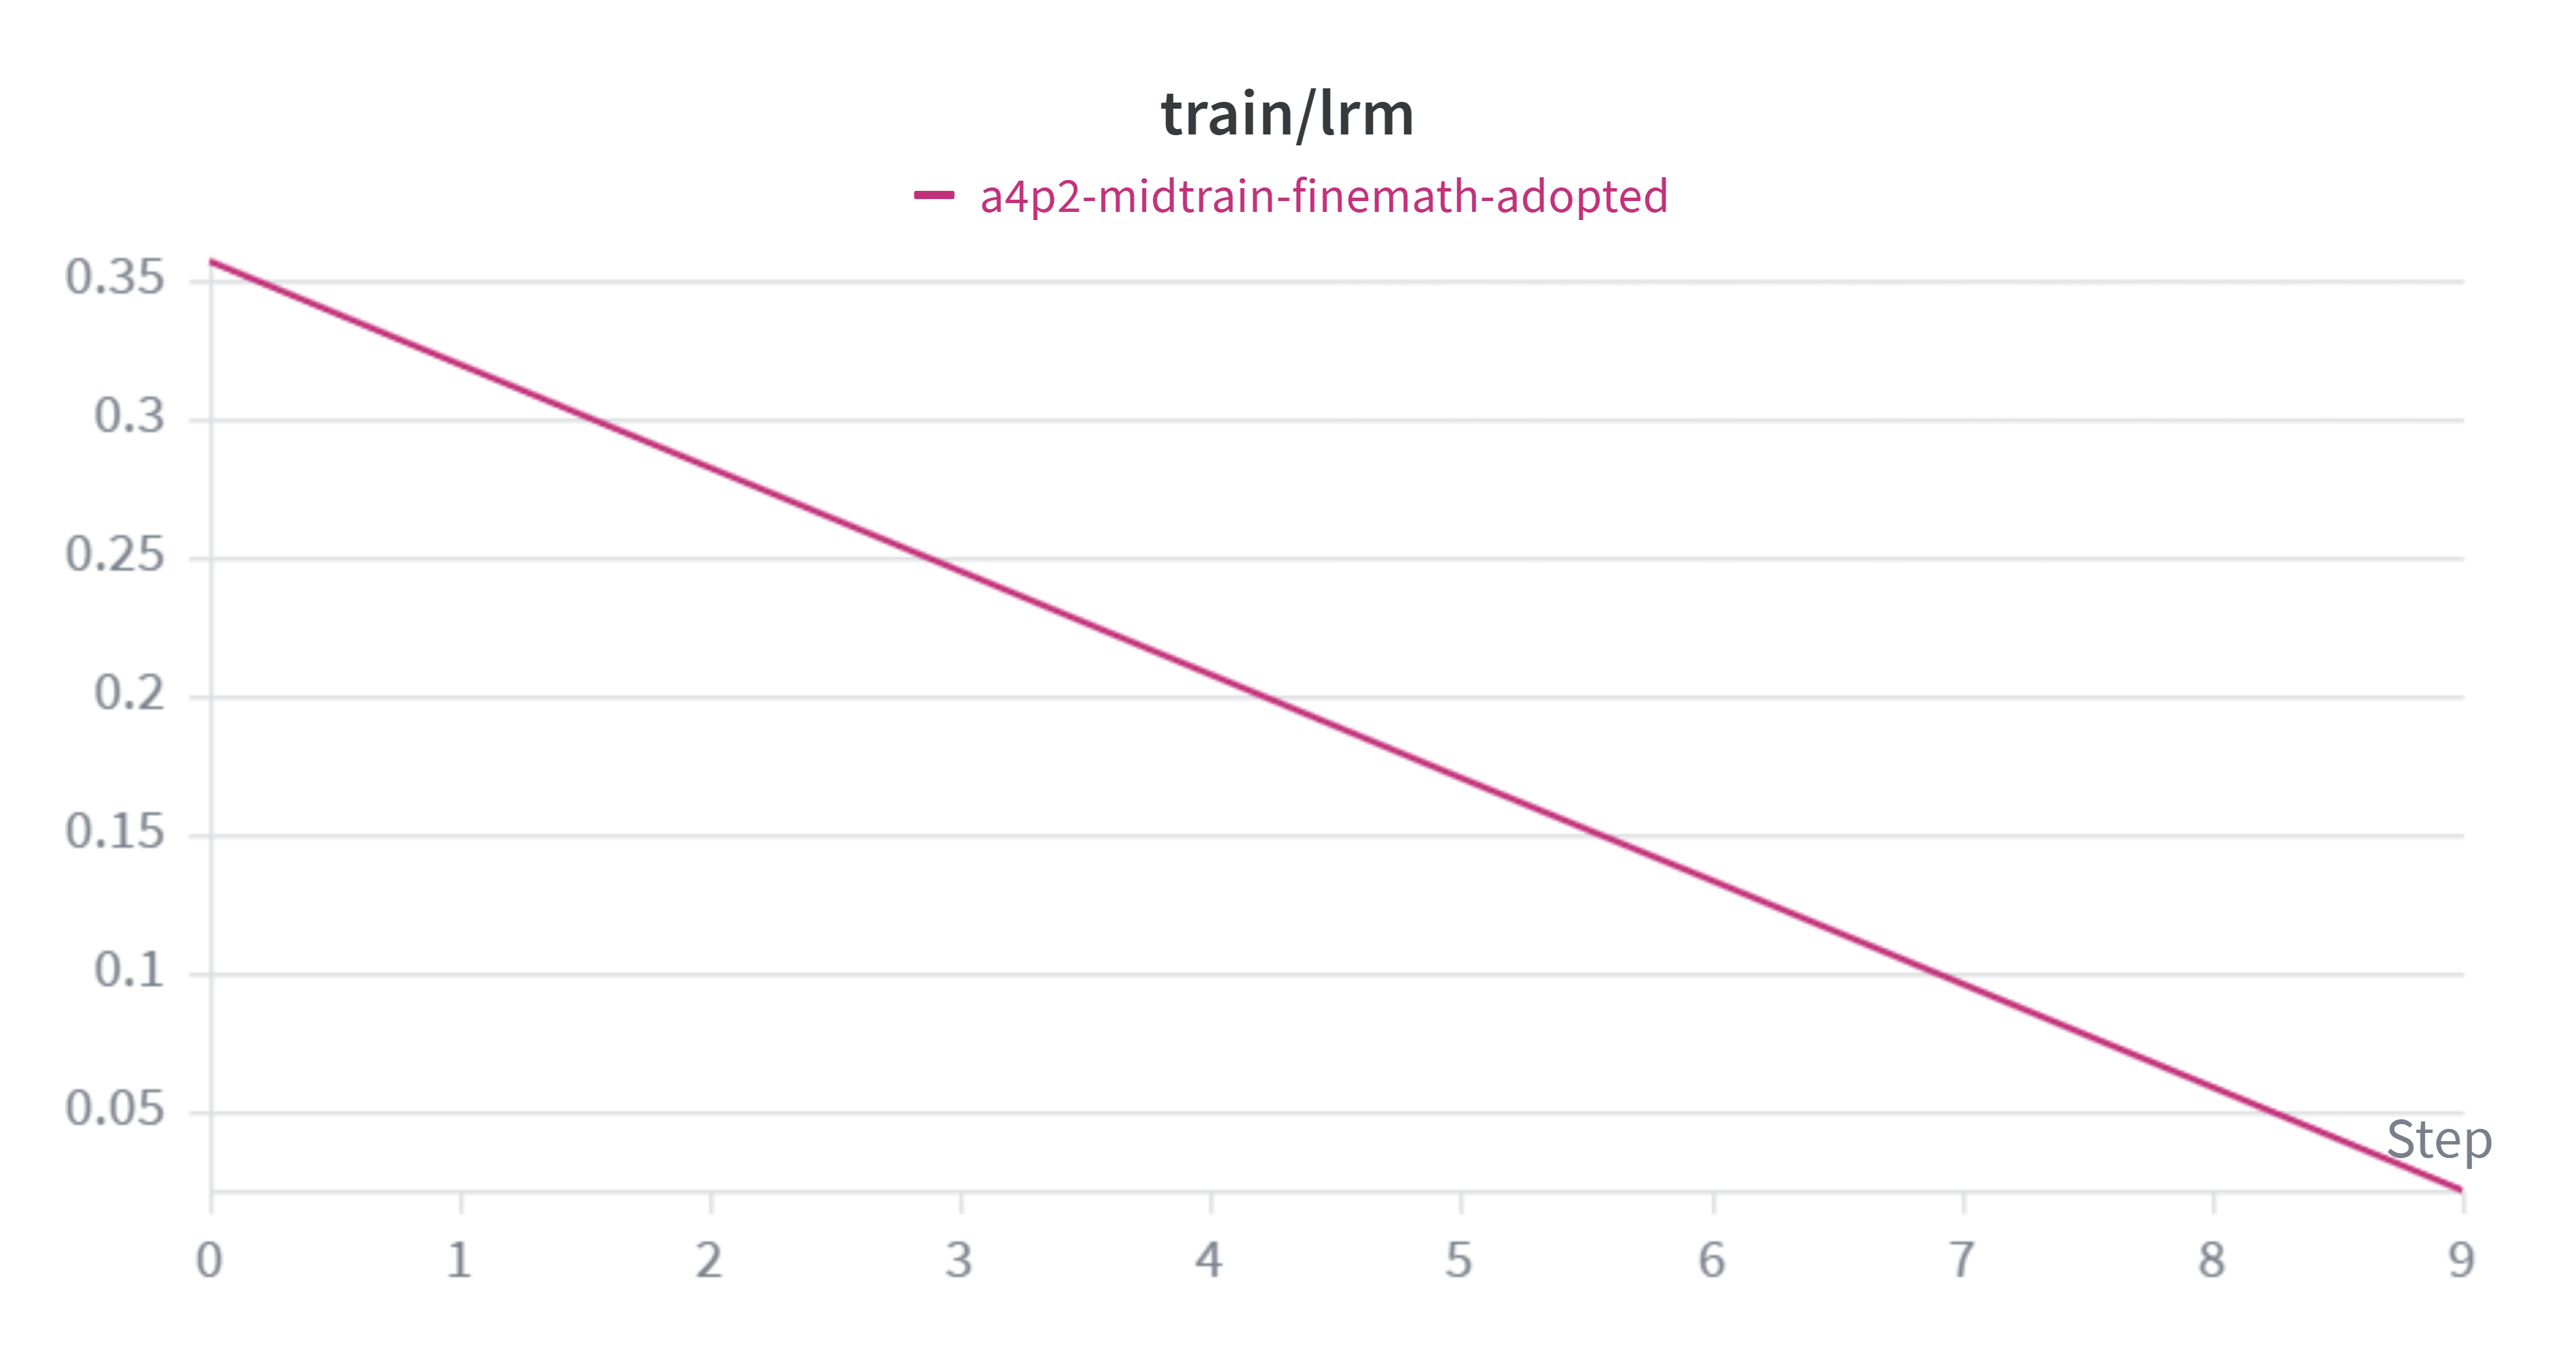
\includegraphics[width=0.75\linewidth]{component/figures/p2/train_math_lr.png}
\caption{Learning rate schedule during midtraining with the FineMath dataset.}
\label{fig:midtrain_lr_compare}
\end{figure}

\paragraph{SFT Training Dynamics.}
The MetaMath SFT run achieves consistently lower training loss than the original SFT
run across the entire training process (Figure~\ref{fig:sft_loss_compare}). The loss
curve for the MetaMath run begins around $1.35$ and gradually decreases to below
$1.0$, whereas the original SFT run starts closer to $1.6$ and remains above roughly
$1.15$ at the end of training. This suggests that the MetaMathQA dataset provides
stronger supervision signals for the instruction-tuning objective.

The learning-rate schedules for both runs follow the same linear decay pattern
(Figure~\ref{fig:sft_lr_compare}). However, the MetaMath run continues for a larger
number of steps, reflecting the longer training duration when the additional dataset
is incorporated.

\paragraph{Midtraining Dynamics.}
A similar pattern appears during midtraining. As shown in
Figure~\ref{fig:midtrain_loss_compare}, the FineMath run exhibits a substantial
reduction in training loss compared with the original midtraining run. The FineMath
model's loss decreases from approximately $2.1$ to below $0.7$ over the course of
training, while the original run remains nearly constant around $2.7$.

The learning rate during the FineMath midtraining run follows the same linear decay
schedule used in the original configuration (Figure~\ref{fig:midtrain_lr_compare}),
indicating that the observed improvement is attributable to the dataset rather than
changes in optimization parameters.

Overall, the training curves indicate that introducing domain-specific mathematical
datasets improves the model's ability to fit the training objective, particularly in
the midtraining stage where the loss decreases substantially relative to the original
run.

\subsubsection{Evaluation Results}

All models were evaluated on the GSM8K benchmark using the same evaluation
pipeline as the original experiments. Table~\ref{tab:extra_results}
summarizes the evaluation metrics, including strict accuracy, relaxed
numeric accuracy, validation bits-per-byte (BPB), and the parseable rate.

\begin{table}[h]
\centering
\caption{GSM8K evaluation results for additional dataset experiments.}
\label{tab:extra_results}
\begin{tabular}{l
                S[table-format=2.2]
                S[table-format=2.2]
                S[table-format=1.3]
                S[table-format=2.2]}
\toprule
\textbf{Model} & \textbf{Strict Acc. (\%)} & \textbf{Relaxed Acc. (\%)} & \textbf{Val BPB} & \textbf{Parseable Rate (\%)} \\
\midrule
Original SFT & 5.23 & 6.37 & 1.5242 & 73.16 \\
MetaMath SFT & \bfseries 15.39 & \bfseries 16.22 & \bfseries 1.520 & \bfseries 88.93 \\
Original Midtraining & 0.00 & 1.06 & \bfseries 0.7753 & 0.00 \\
FineMath Midtraining & 0.00 & 1.90 & 1.7412 & 0.15 \\
\bottomrule
\end{tabular}
\end{table}

The MetaMath SFT model substantially improves performance compared with
the original SFT configuration. Strict accuracy increases from
$5.23\%$ to $15.39\%$, while relaxed numeric accuracy increases from
$6.37\%$ to $16.22\%$. In addition, the parseable rate improves from
$73.2\%$ to $88.9\%$, indicating that the MetaMath dataset helps the
model produce answers in a format that can be interpreted by the
standard GSM8K answer extractor.

For the midtraining stage, both models achieve very low strict accuracy.
However, the FineMath midtraining model slightly improves relaxed
numeric accuracy from $1.06\%$ to $1.90\%$. Despite this improvement,
the parseable rate remains extremely low ($<0.2\%$), which explains
why strict accuracy remains zero. The outputs produced by the model
rarely follow the answer formatting convention required by the
GSM8K evaluation script.

\subsubsection{Comparison with Original Runs}

Comparing the additional dataset experiments with the original training
runs reveals several important patterns:

\begin{itemize}

\item \textbf{MetaMath SFT substantially improves reasoning performance.}
The MetaMathQA dataset increases strict GSM8K accuracy by nearly
three times relative to the original SFT run, suggesting that
instruction tuning on structured mathematical reasoning examples
transfers effectively to GSM8K-style arithmetic problems.

\item \textbf{MetaMath SFT improves answer formatting.}
The parseable rate increases from $73\%$ to nearly $89\%$, indicating
that the model is more likely to produce answers in a format that can
be extracted by the GSM8K evaluation pipeline.

\item \textbf{FineMath midtraining yields limited gains.}
Although the FineMath midtraining run slightly increases relaxed
numeric accuracy, the parseable rate remains extremely low. As a
result, strict accuracy remains zero.

\item \textbf{Answer formatting remains a major bottleneck.}
Many generated responses contain reasoning text but do not present the
final answer in the exact format required by the GSM8K extractor.
This explains the persistent gap between strict and relaxed accuracy.

\end{itemize}

Overall, incorporating domain-specific mathematical datasets improves
instruction-tuned reasoning performance, particularly during SFT.
However, midtraining alone is insufficient to produce reliable
GSM8K-style answers. Additional instruction tuning or reinforcement
learning may be required to enforce consistent reasoning traces and
correct final answer formatting.

\paragraph{Why SFT Improves More Than Midtraining.}

The large improvement observed in the MetaMath SFT run compared with the
FineMath midtraining run can be explained by the difference in training
objectives. Supervised fine-tuning (SFT) directly optimizes the model to
produce structured answers given a prompt–response pair, which aligns
closely with the GSM8K evaluation format. In contrast, midtraining is
performed with a language-modeling objective that focuses on predicting
the next token in general mathematical text. While this objective
improves the model's familiarity with mathematical content, it does not
explicitly teach the model to output a final answer in the structured
format expected by GSM8K. As a result, the SFT stage significantly
improves both accuracy and parseable output rate, whereas midtraining
primarily improves the model's exposure to mathematical concepts without
substantially improving answer formatting. This highlights the
importance of instruction tuning when adapting pretrained language
models to structured reasoning benchmarks.